\sect{Kontextfreie Grammatiken}

Eine \textbf{kontextfreie Grammatik} $G$ (KFG) ist ein 4-Tupel $(N, \Sigma, P, A)$ mit
\begin{itemize}
    \item $N$ ist das Alphabet der \textbf{Nichterminale} (Variablen).
    \item $\Sigma$ ist das Alphabet der \textbf{Terminale}.
    \item $P$ ist eine endliche Menge von \textbf{Produktionen} (Regeln).
    Jede Produktion hat die Form $X \rightarrow \beta$ mit \textbf{Kopf} $X \in N$ und Rumpf $\beta \in (N \cup \Sigma)^*$.
    \item $A$ ist das \textbf{Startsymbol}, wobei $A \in N$.
\end{itemize}

Seien $\alpha$, $\beta$ und $\gamma$ Satzformen und $A \rightarrow \gamma$ eine Produktion.
\begin{itemize}
    \item Durch einen \textbf{Ableitungsschritt} wird eine Satzform $\alpha A \beta$ durch die Anwendung der Produktion $A \rightarrow \gamma$ in die Satzform $\alpha \gamma \beta$ \textbf{abgeleitet}.
    Notation: $\alpha A \beta \Rightarrow \alpha \gamma \beta$
    \item Eine \textbf{Ableitung} ist eine Folge von Ableitungsschritten, sodass aus einer Satzform $\alpha$ das Wort $w$ abgeleitet wird. $\alpha \Rightarrow \dots \Rightarrow w$.
\end{itemize}

\columnbreak

Eine Ableitung kann als \textbf{Ableitungsbaum}/Parsebaum dargestellt werden.
Z.B.\ Ableitungsbaum für das Wort $(())()$.

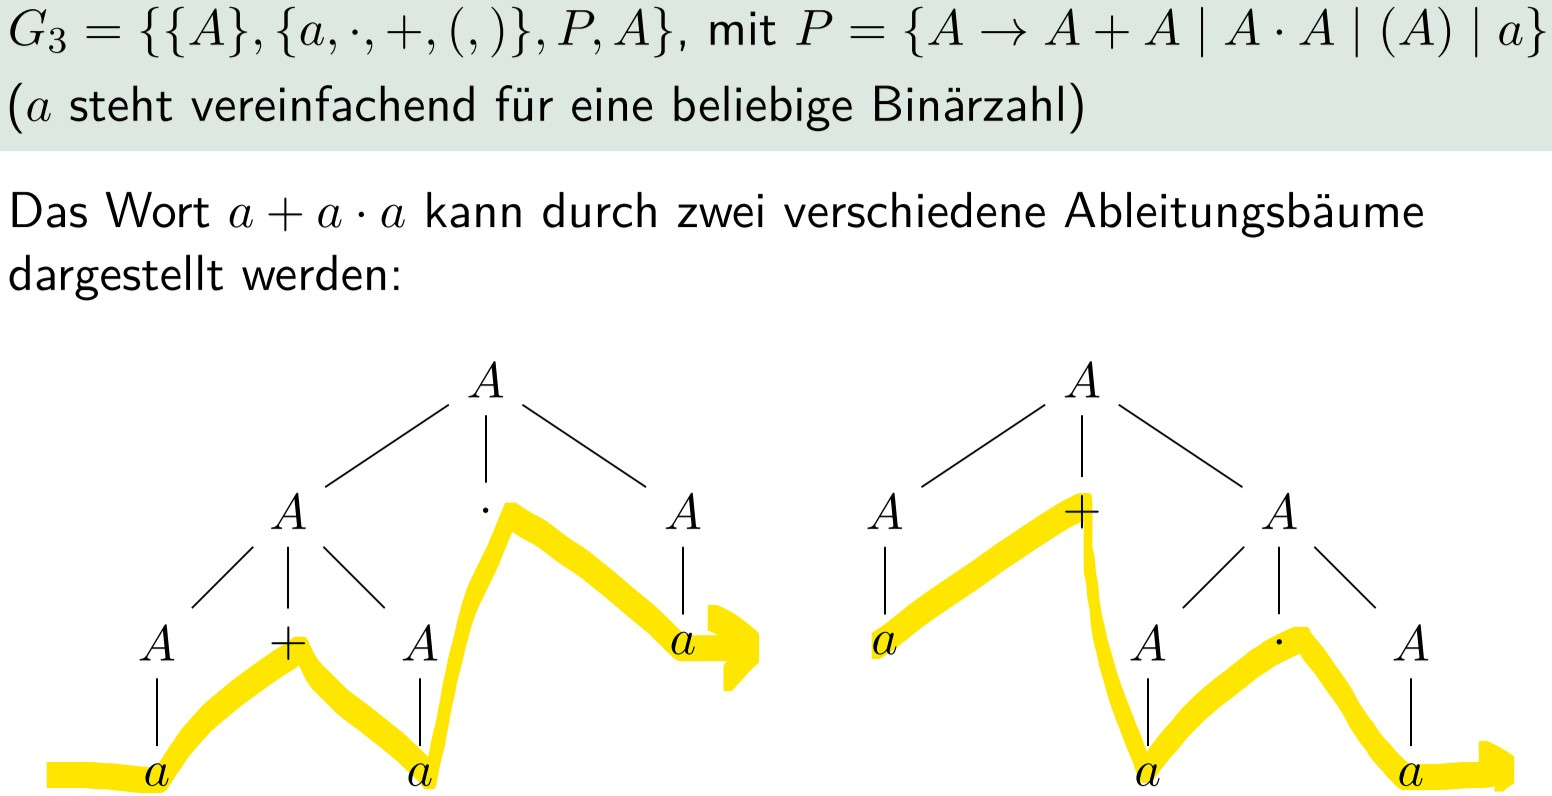
\includegraphics[scale=0.16]{ableitungsbaum}

Eine kontextfreie Grammatik nennen wir \textbf{mehrdeutig}, wenn es ein Wort gibt, das mehrere Ableitungsbäume besitzt.

Mehrdeutigkeit zu verhindern:
\begin{itemize}
    \item Korrekte Klammerung erzwingen
    \item Grammatik anpassen
    \item Den Produktionen Vorrang vergeben
\end{itemize}

Jede reguläre Sprache kann durch eine KFG beschrieben werden.

Sei $L$ eine reguläre Sprache.
Dann gibt es einen DEA $M = (Q, \Sigma, \delta, q_0, F)$ mit $L(M) = L$.
Wir können einen KFG für L wie folgt bauen:
\begin{itemize}
    \item Für jeden Zustand $q_i$ gibt es ein Nichtterminal $Q_i$
    \item Für jede Transition $\delta(q_i, a) = q_j$ erstellen wir die Produktion $Q_i \rightarrow a Q_j$
    \item Für jeden akzeptierenden Zustand $q_i \in F$ erstellen wir die Produktion $Q_i \rightarrow \varepsilon$
    \item Das Nichtterminal $Q_0$ wird zum Startsymbol $A$
\end{itemize}

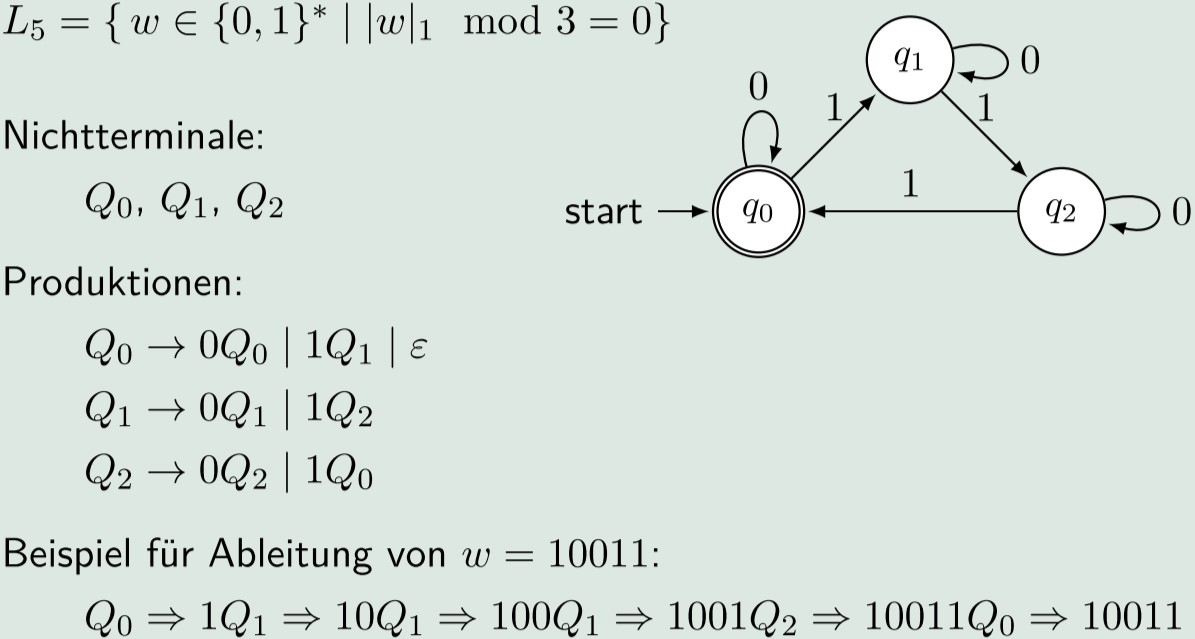
\includegraphics[scale=0.215]{kfg}%